\title{CMPS 240 Artificial Intelligence\\RPS-Safari}
\author{Kerui Huang\\khuang7@ucsc.edu}
\date{\today}
\documentclass[10pt]{article}
\usepackage[cm]{fullpage}
\usepackage{graphicx}
\usepackage{wrapfig}
\usepackage{bm}
\usepackage{amssymb}
\usepackage{amsmath}
\usepackage{epsfig}
\begin{document}
\maketitle

\section{INTRODUCTION}
Rock-paper-scissors (RPS) is a simple game, but it does involve some fundamental problems about the fields of artificial intelligence, such as how to design a decent algorithm to make the computation more intelligent.

Theoretically, if someone is playing RPS completely randomly, it is impossible to gain any advantage against this player. However, human players tend not to be completely random, neither do most machines. Therefore,we are interested in finding a computational method, or say an algorithm, to make an agent computational ``intelligent".

\section{STRATEGY}
\subsection{Why Not Random}
Playing randomly is somehow a good strategy. Because it is random, there is no pattern under the hood to be discovered. At this point, it can successfully confuse opponents. 

However, it also means that it is closed, namely, it does not learn. What if an opponent always plays rock? If the agent perceives it, it can always play paper to beat this opponent. This strategy is apparently better than playing randomly in this case. Actually, as mentioned above, players are usually non-random. In this sense, maybe we can use heuristic algorithms to build a strong agent which is likely to predict others' behavior.

\subsection{My Strategy}

\subsubsection{Choice}
First, the agent should know \textbf{\textit{which one to play}}. Rock, paper or scissor? Since this is a simple agent (first version), I do not apply complicated computations to this problem. The basic idea is that the agent takes all inputs (the number of rock, paper and scissor played each round), sums them up, and calculates its probability to win by playing rock, paper, scissor respectively\footnote{For the first round, since there is no previous information available, the agent just randomly (more precisely, pseudo-randomly) picks up rock, paper or scissor.}. Here is the example:
\begin{quote}
\textbf{Example 1:}\\
Suppose we have ((1 3 4) (8 3 1) (3 4 9)) after 3 rounds. First, the agent takes all the input, and sums them up respectively. Then, the list is flattened as (12 10 14). Therefore, based on this previous experience, the probability \footnote{Maybe not strict ``probability", but it somehow reflects the probability.} for playing rock, paper and scissor are: R = S - P = 4, P = R - S = -2, S = P - R = 2. Therefore, playing R is most possible to win, so the agent plays $R$.
\end{quote}

\subsubsection{Weight}
The second question is \textbf{\textit{how much the agent bets for this round}}. After\footnote{Again, for the first round, the agent just randomly weighs its bet. In addition, the bet surely cannot break  our RPS-Safari rules. Please see the basic requirements on the website.} the first round, the agent knows how it performed in the last round. So here, the idea is to better the weight of its bet according to its past performance. My assumption is:
\begin{quote}
\textbf{Assumption 1:} \textit{If the agent played really well in previous rounds, it makes sense that it should be more confident of itself and then bet more than last round, or vice versa.}
\end{quote}

Besides this reasonable assumption, some other scenarios should be considered. For example, as Prof. Levinson mentioned in the lecture, even though an agent wins every time, it is not a good idea to bet all it has. Once it loses, it loses all. Therefore, my considerations are:
\begin{quote}
\begin{itemize}
\item \textbf{Case 1:} When an agent gains a very high score, it is good to be more conservative, because the important thing is to keep its upper hand. ``Conservative" means it almost keeps its old weight, not increases it dramatically any more.
\item \textbf{Case 2:} When an agent gains a somewhat high score and it keeps performing very well, since it has not reached a very high score, it is advisable to let it be more aggressive and consequently add more weight to its bet in order to make improvements faster.
\item \textbf{Case 3:} When an agent just starts its adventure or it played so far neither too bad nor very well, it had better be conservative and wait until it gains more experience after rounds. When it performs better and better (Case 2), it can begin to bet more.
\item \textbf{Case 4:} So far, I only discussed about the scenarios in which an agent plays not bad. What if the agent plays very bad? If an agent plays bad, it sort of means that it cannot trust itself. However, it is still helpful, because it can just take the opposite decision. So, bad cases become simple -- the agent just reverses its original choice (which is made based on the first three cases).
\end{itemize}
\end{quote}

Then, to formulate these behaviors, my agent utilizes the formulae \footnote{Note that this formula only can be applied to the cases when the agent plays well. If the agent plays bad, just change the sign of value returned by this function.} as follows:
$$
weight=ceiling(f(x))
$$
$$
f(x)=10\times arctan(.05\times (x - 100)) + 14, when\ score\geq 0
$$
where $x$ is the current score of the agent.

The term 10 controls the scale of the weight, since the original $arctan$ function is too small to fit our score scale. The term .05 controls how fast the agent increase the weight of its play. The term 100 means the point at which the agent thinks it should make the fastest improvement. Namely, when the agent reaches 100 points, the increment of the weight is largest.

The term 14 is used for bounding the absolute value of the weight. Because 
$$
\lim_{x \to -\infty} (10\times arctan(.05\times (x - 100))) = -15.708
$$ and we need to make sure the bet is positive \footnote{Here we consider positive cases only. For negative cases, we will simply change the sign later.}, we need to add 14 to ensure it is positive when score is 0.

Figure \ref{figure:a} shows the change of the weight for positive cases.

\begin{figure}
\centering
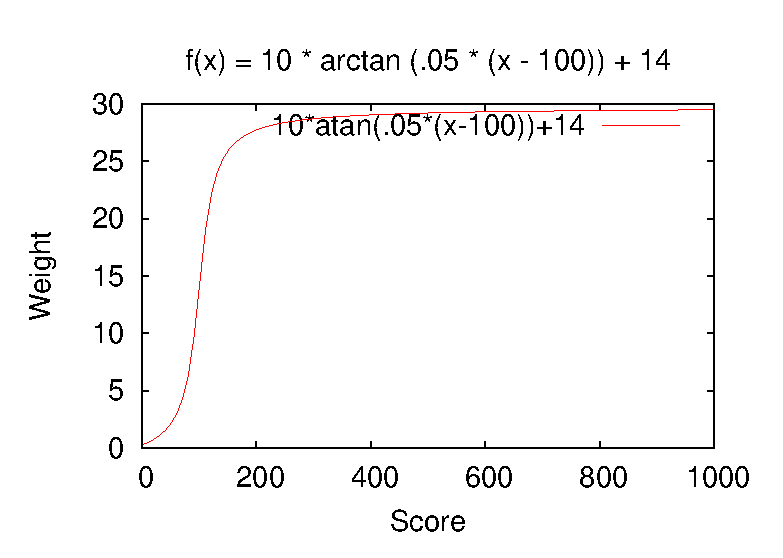
\epsfig{file=b.eps, height=2in, width=2.5in}
\caption{The function $f(x)=10\times arctan(.05\times (x - 100)) + 14, when\ score\geq 0$}
\label{figure:a}
\end{figure}

%\begin{table}
%\caption{Comparing early result rates.($c=\frac{|A||B|M}{(|A|+|B|)^2FT}$)}
%\label{tab:rrcomp}
%\center
%\begin{tabular}{|c|c|} \hline
%& $F=1.2, T_{ri}=T_{wt}=T_{rt}=T$ \\ \hline
%Symmetric Hash & $c$ (Must fit in memory)\\ \hline
%Hash Ripple & $ 0.5c $ \\ \hline
%SMS-Join & $ 0.6c $ \\ \hline
%Block Ripple & $ \frac{2k+1}{k+2}c:c, 1.25c, 1.40c, ... $ \\ \hline
%PR-Join ($ \gamma=1 $) & $ c, 1.7c, 3.2c, 6.2c, 12.2c, ... $ \\ \hline
%\end{tabular}
%\end{table}

%\begin{figure}
%\centering
%\includegraphics[width=50mm]{size.jpeg}
%\caption{A 10G relation joins a 20G relation}
%\label{figure:size}
%\end{figure}
%\bibliographystyle{abbrv}
%\bibliography{bib}
\end{document} 
